\newpage
\section{Các công thức lượng giác}
\subsection{Lý thuyết cần nhớ}
\subsubsection{Công thức cộng}
\begin{multicols}{2}
	\begin{itemize}
		\item $\sin (\alpha + \beta)=\sin \alpha\cos \beta+ \sin \beta\cos \alpha$.
		\item $\sin (\alpha - \beta)=\sin \alpha\cos \beta-\sin \beta\cos \alpha$.
		\item $\cos (\alpha + \beta)=\cos \alpha\cos \beta - \sin \alpha\sin \beta$.
		\item $\cos (\alpha - \beta)=\cos \alpha\cos \beta +\sin \alpha\sin \beta$.
		\item $\tan (\alpha + \beta)=\dfrac{\tan \alpha + \tan \beta}{1-\tan \alpha\tan \beta}$.
		\item $\tan (\alpha - \beta)=\dfrac{\tan \alpha - \tan \beta}{1+\tan \alpha\tan \beta}$.
	\end{itemize}
\end{multicols}
\subsubsection{Công thức góc nhân đôi}
\begin{itemize}
	\item $\cos2\alpha = \cos^2\alpha - \sin^2\alpha = 2\cos^2\alpha - 1 = 1 - 2\sin^2\alpha$.
	\item $\sin2\alpha=2\sin \alpha\cos \alpha$.
	\item $\tan2\alpha=\dfrac{2\tan \alpha}{1-\tan^2\alpha}$.
\end{itemize}
\begin{nx}
$\cos ^{2} a=\dfrac{1+\cos 2 a}{2}$; $\sin ^{2} a=\dfrac{1-\cos 2 a}{2}$ (thường gọi là công thức hạ bậc).
\end{nx}
\subsubsection{Công thức biến đổi tích thành tổng}
\begin{itemize}
		\item  $\cos \alpha\cos \beta=\dfrac{1}{2}\left[\cos \left({\alpha - \beta}\right)+\cos \left({\alpha + \beta}\right)\right]$;
		\item  $\sin \alpha\sin \beta=\dfrac{1}{2}\left[{\cos\left({\alpha - \beta}\right) - \cos\left({\alpha + \beta}\right)}\right]$;
		\item  $\sin \alpha\cos \beta=\dfrac{1}{2}\left[{\sin\left({\alpha - \beta}\right) + \sin\left({\alpha + \beta}\right)}\right]$.
\end{itemize}
\subsubsection{Công thức biến đổi tổng thành tích}
	\begin{multicols}{2}
		\begin{itemize}
			\item  $\cos \alpha + \cos \beta = 2\cos \dfrac{{\alpha + \beta}}{2}\cos \dfrac{{\alpha - \beta}}{2}$;
			\item  $\cos \alpha - \cos \beta = -2\sin\dfrac{{\alpha + \beta}}{2}\sin\dfrac{{\alpha - \beta}}{2}$;
			\item  $\sin \alpha + \sin \beta = 2\sin \dfrac{{\alpha + \beta}}{2}\cos \dfrac{{\alpha - \beta}}{2}$;
			\item  $\sin \alpha-\sin \beta=2\cos\dfrac{{\alpha + \beta}}{2}\sin\dfrac{{\alpha - \beta}}{2}$.
		\end{itemize}
	\end{multicols}
\subsection{Phân loại và phương pháp giải toán}

\begin{dang}{Công thức cộng}
\textbf{Công thức cộng}
\begin{multicols}{2}
	\begin{itemize}
		\item $\sin (\alpha + \beta)=\sin \alpha\cos \beta+ \sin \beta\cos \alpha$.
		\item $\sin (\alpha - \beta)=\sin \alpha\cos \beta-\sin \beta\cos \alpha$.
		\item $\cos (\alpha + \beta)=\cos \alpha\cos \beta - \sin \alpha\sin \beta$.
		\item $\cos (\alpha - \beta)=\cos \alpha\cos \beta +\sin \alpha\sin \beta$.
		\item $\tan (\alpha + \beta)=\dfrac{\tan \alpha + \tan \beta}{1-\tan \alpha\tan \beta}$.
		\item $\tan (\alpha - \beta)=\dfrac{\tan \alpha - \tan \beta}{1+\tan \alpha\tan \beta}$.
	\end{itemize}
\end{multicols}
\end{dang}

\begin{vd}%[1D1N3-2]%[Dự án đề cương 3 Khối NH 24-25- Dot 3- Nguyễn Trần Anh Tuấn]
	Tính
	\begin{multicols}{2}
		\begin{enumerate}
			\item $\sin 75^{\circ}$.
			\item $\sin \dfrac{\pi}{12}$.
		\end{enumerate}
	\end{multicols}
	\loigiai{
		\begin{enumerate}
			\item Áp dụng công thức cộng, ta có\\
			$\sin 75^{\circ}=\sin \left(30^{\circ}+45^{\circ}\right)=\sin 30^{\circ} \cos 45^{\circ}+\cos 30^{\circ} \sin 45^{\circ}=\dfrac{\sqrt{6}+\sqrt{2}}{4}$.
			\item Áp dụng công thức cộng, ta có\\
			$\sin \dfrac{\pi}{12}=\sin \left(\dfrac{\pi}{3}-\dfrac{\pi}{4}\right)=\sin \dfrac{\pi}{3} \cos \dfrac{\pi}{4}-\cos \dfrac{\pi}{3} \sin \dfrac{\pi}{4}=\dfrac{\sqrt{6}-\sqrt{2}}{4}$.
		\end{enumerate}
	}
\end{vd}

\begin{vd}%[1D1H3-2]%[Dự án đề cương 3 Khối NH 24-25- Dot 3- Nguyễn Trần Anh Tuấn]
	Chứng minh rằng $\sin x+\cos x=\sqrt{2} \sin \left(x+\dfrac{\pi}{4}\right)$.
	\loigiai{
		Ta có
		\[\begin{aligned}
		\sqrt{2} \sin \left(x+\dfrac{\pi}{4}\right)
		&=\sqrt{2}\left(\sin x \cos \dfrac{\pi}{4}+\cos x \sin \dfrac{\pi}{4}\right)\\
		&=\sqrt{2}\left(\sin x \cdot \dfrac{\sqrt{2}}{2}+\cos x \cdot \dfrac{\sqrt{2}}{2}\right)\\
		&=\sin x+\cos x.
		\end{aligned}\]
		Đẳng thức được chứng minh.
	}
\end{vd}

\begin{dang}{Công thức nhân đôi, công thức hạ bậc}
 \begin{itemize}
	\item $\cos2\alpha = \cos^2\alpha - \sin^2\alpha = 2\cos^2\alpha - 1 = 1 - 2\sin^2\alpha$.
	\item $\sin2\alpha=2\sin \alpha\cos \alpha$.
	\item $\tan2\alpha=\dfrac{2\tan \alpha}{1-\tan^2\alpha}$.
\end{itemize}

\begin{nx}
$\cos ^{2} a=\dfrac{1+\cos 2 a}{2}$; $\sin ^{2} a=\dfrac{1-\cos 2 a}{2}$ (thường gọi là công thức hạ bậc).
\end{nx}   
\end{dang}

\begin{vd}%[1D1H3-3]%[Dự án đề cương 3 Khối NH 24-25- Dot 3- Nguyễn Trần Anh Tuấn]
	Cho $\sin a+\cos a=\dfrac{1}{2}$. Tính $\sin 2 a$, $\cos 4 a$.		
	\loigiai{
		\begin{itemize}
			\item Do $\sin a+\cos a=\dfrac{1}{2}$ nên 
				\begin{eqnarray*}
					&&(\sin a+\cos a)^{2}=\dfrac{1}{4} \\
					&\Leftrightarrow& \sin ^{2} a+\cos ^{2} a+2 \sin a \cos a=\dfrac{1}{4}\\
					&\Leftrightarrow& 1+2 \sin a \cos a=\dfrac{1}{4}\\
					&\Leftrightarrow& \sin 2 a=\dfrac{1}{4}-1=-\dfrac{3}{4}.
				\end{eqnarray*}
			\item Áp dụng công thức nhân đôi, ta có $\cos 4 a=\cos (2 \cdot 2 a)=1-2 \sin ^{2} 2 a=-\dfrac{1}{8}$.
		\end{itemize}
	}
\end{vd}
\begin{vd}%[1D1N3-3]%[Dự án đề cương 3 Khối NH 24-25- Dot 3- Nguyễn Trần Anh Tuấn]
	Cho $\tan \dfrac{a}{2}=-2$. Tính $\tan a$.
	\loigiai{
		Áp dụng công thức nhân đôi, ta có
		$$\tan a=\dfrac{2 \tan\dfrac{a}{2}}{1-\tan ^2 \dfrac{a}{2}}=\dfrac{2 \cdot (-2)}{1-(-2)^2}=-\dfrac{4}{3}.$$
	}
\end{vd}

\begin{dang}{Công thức biến đổi tích thành tổng}
\begin{itemize}
		\item  $\cos \alpha\cos \beta=\dfrac{1}{2}\left[\cos \left({\alpha - \beta}\right)+\cos \left({\alpha + \beta}\right)\right]$;
		\item  $\sin \alpha\sin \beta=\dfrac{1}{2}\left[{\cos\left({\alpha - \beta}\right) - \cos\left({\alpha + \beta}\right)}\right]$;
		\item  $\sin \alpha\cos \beta=\dfrac{1}{2}\left[{\sin\left({\alpha - \beta}\right) + \sin\left({\alpha + \beta}\right)}\right]$.
\end{itemize}
\end{dang}

\begin{vd}%[1D1N3-4]%[Dự án đề cương 3 Khối NH 24-25- Dot 3- Nguyễn Trần Anh Tuấn]
	Biết $\sin (a+b)=1$, $\sin (a-b)=\dfrac{1}{2}$. Tính $\sin a\cos b$.
	\loigiai{
		Ta có $\sin a\cos b=\dfrac{1}{2}\left[\sin (a-b)+\sin (a+b)\right]=\dfrac{1}{2}\left(\dfrac{1}{2}+1\right)=\dfrac{3}{4}$.
	}
\end{vd}

\begin{vd}%[1D1H3-4]%[Dự án đề cương 3 Khối NH 24-25- Dot 3- Nguyễn Trần Anh Tuấn]
	Cho $\cos a=\dfrac{2}{3}$. Tính $B=\cos \dfrac{3 a}{2} \cos \dfrac{a}{2}$.
	\loigiai{
		Ta có $\cos2a=2\cos^2 a-1=-\dfrac{1}{9}$.\\
		Do đó
		$$B=\cos \dfrac{3 a}{2} \cos \dfrac{a}{2}=\dfrac{1}{2}\left[\cos \left(\dfrac{3 a}{2}+\dfrac{a}{2}\right)+\cos \left(\dfrac{3 a}{2}-\dfrac{a}{2}\right)\right]=\dfrac{1}{2}\left(\cos 2a+\cos a \right)=\dfrac{5}{18}.
		$$
	}
\end{vd}

\begin{vd}%[1D1H3-4]%[Dự án đề cương 3 Khối NH 24-25- Dot 3- Nguyễn Trần Anh Tuấn]
	Biến đổi thành tổng các biểu thức sau
	\begin{multicols}{2}
		\begin{enumerate}
			\item $A= \sin 5x\cos 3x$.
			\item $B=\sin (x+y) \cos (x-y)$.
		\end{enumerate}
	\end{multicols}
	\loigiai{
		\begin{enumerate}
			\item $A= \sin 5x\cos 3x= \dfrac{1}{2}\left( \sin 2x + \sin 8x\right)$.
			\item $B=\sin (x+y) \cos (x-y)= \dfrac{1}{2}\left( \sin 2y+ \sin 2x\right)$.
		\end{enumerate}
	}
\end{vd}

\begin{dang}{Công thức biến đổi tổng thành tích}
	\begin{multicols}{2}
		\begin{itemize}
			\item  $\cos \alpha + \cos \beta = 2\cos \dfrac{{\alpha + \beta}}{2}\cos \dfrac{{\alpha - \beta}}{2}$;
			\item  $\cos \alpha - \cos \beta = -2\sin\dfrac{{\alpha + \beta}}{2}\sin\dfrac{{\alpha - \beta}}{2}$;
			\item  $\sin \alpha + \sin \beta = 2\sin \dfrac{{\alpha + \beta}}{2}\cos \dfrac{{\alpha - \beta}}{2}$;
			\item  $\sin \alpha-\sin \beta=2\cos\dfrac{{\alpha + \beta}}{2}\sin\dfrac{{\alpha - \beta}}{2}$.
		\end{itemize}
	\end{multicols}
\end{dang}

\begin{vd}%[1D1N3-4]%[Dự án đề cương 3 Khối NH 24-25- Dot 3- Nguyễn Trần Anh Tuấn]
	Tính $\cos \dfrac{7 \pi}{12} + \cos \dfrac{\pi}{12}$.
	\loigiai{
		Ta có $\cos \dfrac{7 \pi}{12} + \cos \dfrac{\pi}{12} = 2\cos \dfrac{\dfrac{7 \pi}{12} + \dfrac{\pi}{12}}{2} \cos \dfrac{\dfrac{7 \pi}{12} - \dfrac{\pi}{12}}{2} = 2 \cos \dfrac{\pi}{3} \cos \dfrac{\pi}{4} = 2 \cdot \dfrac{1}{2} \cdot \dfrac{\sqrt{2}}{2} = \dfrac{\sqrt{2}}{2}.$
	} 
\end{vd}
\begin{vd}%[1D1V3-4]%[Dự án đề cương 3 Khối NH 24-25- Dot 3- Nguyễn Trần Anh Tuấn]
	Rút gọn biểu thức: $A=\dfrac{\sin x+\sin 2 x+\sin 3 x}{\cos x+\cos 2 x+\cos 3 x}$.
	\loigiai{
		$A=\dfrac{(\sin x+\sin 3x)+\sin 2x}{(\cos x+\cos 3x)+\cos 2x}=\dfrac{2\sin2x\cos x+\sin 2x}{2\cos 2x\cos x+\cos 2x}=\dfrac{\sin 2x(2\cos x+1)}{\cos 2x(2\cos x+1)}=\tan 2x$.
	}
\end{vd}

\subsection{Bài tập rèn luyện}
\ind{PHẦN I.} \inden{Câu trắc nghiệm nhiều phương án lựa chọn. Mỗi câu hỏi học sinh chỉ chọn một phương án.}\\
\setcounter{ex}{0}
\Opensolutionfile{ans}[ans/1D1-Bai3-TN]

\begin{ex}[Trích đề thi giữa HKI - THPT Ngô Gia Tự, Đắk Lắk - năm học 2024-2025]%[1D1N3-3]%[Dự án đề cương 3 Khối NH 24-25- Dot 3- Nguyễn Trần Anh Tuấn]
	Công thức nào sau đây là đúng?
	\choice
	{$\cos 2a=\cos a-\sin a$}
	{$\cos 2a=2 \cos a$}
	{$\cos 2a=\cos^2 a+\sin^2 a$}
	{\True $\cos 2a=\cos^2 a-\sin^2 a$}
	\loigiai{
		Công thức nhân đôi $\cos 2a=\cos^2 a-\sin^2 a=1-2\sin^2 a=2\cos^2 a -1$.
	}
\end{ex}

\begin{ex}%[1D1N3-3]%[Dự án đề cương 3 Khối NH 24-25- Dot 3- Nguyễn Trần Anh Tuấn]
	Mệnh đề nào sau đây {\bf sai}?
	\choice
	{$\cos 2a=1-2\sin^2 a$}
	{$\cos 2a=2\cos^2 a-1$}
	{$\cos 2a=\cos^2 a-\sin^2 a$}
	{\True $\cos 2a=\cos^2 a+\sin^2 a$}
	\loigiai{
		$\cos 2a=\cos^2 a+\sin^2 a$ là công thức sai.
	}
\end{ex}

\begin{ex}[Trích đề thi giữa HKI - THPT Chuyên Bình Thuận - năm học 2024-2025]%[1D1N3-4]
	Trong các khẳng định sau, khẳng định nào đúng?
	\choice
	{\True $\sin a-\sin b=2\cos\dfrac{a+b}{2}\sin\dfrac{a-b}{2}$}
	{$\sin a-\sin b=2\sin\dfrac{a+b}{2}\sin\dfrac{a-b}{2}$}
	{$\sin a-\sin b=2\sin\dfrac{a+b}{2}\cos\dfrac{a-b}{2}$}
	{$\sin a-\sin b=2\cos\dfrac{a+b}{2}\cos\dfrac{a-b}{2}$}
	\loigiai{
		Từ công thức biến đổi tổng thành tích, suy ra $\sin a-\sin b=2\cos\dfrac{a+b}{2}\sin\dfrac{a-b}{2}$.
	}
\end{ex}

\begin{ex}%[1D1N3-4]%[Dự án đề cương 3 Khối NH 24-25- Dot 3- Nguyễn Trần Anh Tuấn]
	$2\sin \left(\dfrac{a+b}{2}\right)\cos\left(\dfrac{b-a}{2}\right)$ bằng
	\choice
	{$\cos a+\cos b$}
	{$\sin b-\sin a$}
	{\True $\sin a+\sin b$}
	{$\sin a-\sin b$}
	\loigiai{
		Ta có $\sin a+\sin b =2\sin \left(\dfrac{a+b}{2}\right)\cos\left(\dfrac{b-a}{2}\right)$.
	}
\end{ex}

\begin{ex}[Trích đề thi giữa HKI - THPT Tân Châu, An Giang - năm học 2024-2025]%[1D1N3-1]%[Dự án đề cương 3 Khối NH 24-25- Dot 3- Nguyễn Trần Anh Tuấn]
	Trong các công thức sau, công thức nào \textbf{đúng}?
	\choice
	{$\tan(a-b)=\dfrac{\tan a+\tan b}{1-\tan a \tan b}$} % Giữ nguyên dạng sai trong hình để so sánh
	{$\tan(a+b)=\tan a+\tan b$}
	{\True $\tan(a+b)=\dfrac{\tan a+\tan b}{1-\tan a \tan b}$}
	{$\tan(a-b)=\tan a-\tan b$} % Giữ nguyên dạng sai trong hình để so sánh
	\loigiai{
		Ta có 
		\allowdisplaybreaks
		\begin{eqnarray*}
			\tan(a+b) &=& \dfrac{\tan a+\tan b}{1-\tan a \tan b}\\
			\tan(a-b) &=& \dfrac{\tan a-\tan b}{1+\tan a \tan b}.
		\end{eqnarray*}
	}
\end{ex}

\begin{ex}%[1D1H2-2]%[Dự án đề cương 3 Khối NH 24-25- Dot 3- Nguyễn Trần Anh Tuấn]
	Cho $\sin \alpha=\dfrac{2}{3}$. Tính $\cos 2\alpha$.
	\choice
	{$-\dfrac{1}{9}$}
	{$\dfrac{1}{3}$}
	{$-\dfrac{1}{3}$}
	{\True $\dfrac{1}{9}$}
	\loigiai{
		Ta có $\cos 2\alpha=1-2\sin^2\alpha=1-2\cdot \left(\dfrac{2}{3}\right)^2=\dfrac{1}{9}$.
	}
\end{ex}

\begin{ex}%[1D1H3-3]%[Dự án đề cương 3 Khối NH 24-25- Dot 3- Nguyễn Trần Anh Tuấn]
	Nếu $\cos \alpha =\dfrac{1}{4}$ thì $\cos 2\alpha$ bằng
	\choice
	{$\dfrac{7}{8}$}
	{\True $-\dfrac{7}{8}$}
	{$\dfrac{15}{16}$}
	{$-\dfrac{15}{16}$}
	\loigiai{
		Ta có $\cos 2\alpha = 2\cos^2 \alpha-1=2\cdot \left(\dfrac{1}{4}\right)^2-1=-\dfrac{7}{8}$.
	}
\end{ex}

\begin{ex}[Trích đề thi giữa HKI - THPT Nguyễn Thị Minh Khai, Tp HCM - năm học 2024-2025]%[1D1N3-4]%[Dự án đề cương 3 Khối NH 24-25- Dot 3- Nguyễn Trần Anh Tuấn]
	Với mọi góc lượng giác $a$ và $b$, khẳng định nào sau đây là \textbf{sai}?
	\choice
	{$\cos a+\cos b=2\cos \dfrac{a+b}{2}\cdot\cos \dfrac{a-b}{2}$}
	{\True $\cos a-\cos b=2\sin \dfrac{a+b}{2}\cdot\sin \dfrac{a-b}{2}$}
	{$\sin a+\sin b=2\sin \dfrac{a+b}{2}\cdot\cos \dfrac{a-b}{2}$}
	{$\sin a-\sin b=2\cos \dfrac{a+b}{2}\cdot\sin \dfrac{a-b}{2}$}
	\loigiai{
	Ta có $\cos a-\cos b=-2\sin \dfrac{a+b}{2}\cdot\sin \dfrac{a-b}{2}$	
	}
\end{ex}

\begin{ex}%[1D1H3-3]%[Dự án đề cương 3 Khối NH 24-25- Dot 3- Nguyễn Trần Anh Tuấn]
	Cho $\cos{x}=\dfrac{4}{5}$, $x\in \left(-\dfrac{\pi}{2};0 \right)$. Giá trị của $\sin{2x}$ là
	\choice
	{\True $-\dfrac{24}{25}$}
	{$\dfrac{24}{25}$}
	{$\dfrac{1}{5}$}
	{$-\dfrac{1}{5}$}
	\loigiai{
		Vì $x\in \left(-\dfrac{\pi}{2};0 \right)$ nên $\sin{x}=-\sqrt{1^2-\cos^2{x}}=-\sqrt{1-\left(\dfrac{4}{5} \right)^2}=-\dfrac{3}{5}$.\\ 
		Suy ra $\sin{2x}=2\sin{x} \cos{x}=2\cdot \left(-\dfrac{3}{5} \right)\cdot \dfrac{4}{5}=-\dfrac{24}{25}$.
	}
\end{ex}

\begin{ex}%[1D1N3-2]%[Dự án đề cương 3 Khối NH 24-25- Dot 3- Nguyễn Trần Anh Tuấn]
	Cho $\sin \alpha \cdot \cos \beta=\dfrac{1}{2}$ và $\cos \alpha \cdot \sin \beta=\dfrac{1}{3}$. Tính $\sin (\alpha+\beta)$.
	\choice
	{\True $\sin (\alpha+\beta)=\dfrac{5}{6}$}
	{$\sin (\alpha+\beta)=\dfrac{2}{3}$}
	{$\sin (\alpha+\beta)=\dfrac{1}{6}$}
	{$\sin (\alpha+\beta)=-\dfrac{1}{6}$}
	\loigiai{
		Ta có $\sin (\alpha +\beta)=\sin \alpha \cos \beta +\cos \alpha \sin \beta =\dfrac{1}{2}+\dfrac{1}{3}=\dfrac{5}{6}$.
	}
\end{ex}

\begin{ex}%[1D1H3-2]%[Dự án đề cương 3 Khối NH 24-25- Dot 3- Nguyễn Trần Anh Tuấn]
	Rút gọn $M=\cos (a+b)\cos (a-b)-\sin (a+b)\sin (a-b)$.
	\choice
	{$M=\sin 4a$}
	{$M=\cos 4a$}
	{\True $M=1-2\sin^2a$}
	{$M=1-2\cos^2a$}
	\loigiai
	{
		Ta có $M=\cos \left(a+b+a-b\right)=\cos 2a=1-2\sin^2a$.
	}
\end{ex}

\begin{ex}%[1D1H3-2]%[Dự án đề cương 3 Khối NH 24-25- Dot 3- Nguyễn Trần Anh Tuấn]
	Cho $\sin a=\dfrac{5}{13}$, $\cos a=\dfrac{12}{13}$; $\sin b=\dfrac{4}{5}$ và $\cos b =\dfrac{3}{5}$. Khẳng định nào sau đây đúng?
	\choice
	{$\cos (a+b)=\dfrac{56}{65}$}
	{\True  $\cos (a+b)=\dfrac{16}{65}$}
	{$\cos (a+b)=-\dfrac{33}{65}$}
	{$\cos (a+b)=\dfrac{63}{65}$}
	\loigiai{
		Ta có $\cos (a+b) =\cos a \cos b - \sin a\sin b = \dfrac{12}{13} \cdot \dfrac{3}{5} -\dfrac{5}{13} \cdot  \dfrac{4}{5}=\dfrac{16}{65}$.
	}
\end{ex}

\begin{ex}%[1D1H3-3]%[Dự án đề cương 3 Khối NH 24-25- Dot 3- Nguyễn Trần Anh Tuấn]
	Biết $\cos 2 a=\dfrac{1}{3}$. Giá trị của $\cos 4 a$ bằng
	\choice
	{$-\dfrac{1}{3}$}
	{$\dfrac{2}{3}$}
	{$\dfrac{7}{9}$}
	{\True $-\dfrac{7}{9}$}
	\loigiai{
		$\cos 4a=2\cos^2 2a	-1=2\cdot \dfrac{1}{9}-1=-\dfrac{7}{9}$.
	}
\end{ex}

\begin{ex}%[1D1H3-3]%[Dự án đề cương 3 Khối NH 24-25- Dot 3- Nguyễn Trần Anh Tuấn]
	Cho $\cos \alpha=\dfrac{4}{5}$. Tính $\cos 2 \alpha$.
	\choice
	{$-\dfrac{7}{25}$}
	{\True $\dfrac{7}{25}$}
	{$-\dfrac{24}{25}$}
	{$\dfrac{24}{25}$}
	\loigiai{
		Ta có $\cos 2\alpha=2\cos^2\alpha-1=\dfrac{7}{25}$.
	}
\end{ex}

\begin{ex}%[1D1H3-4]%[Dự án đề cương 3 Khối NH 24-25- Dot 3- Nguyễn Trần Anh Tuấn]
	Biết $\cos(a+b)=\dfrac{\sqrt{3}}{2}$, $\cos(a-b)=\dfrac{1}{2}$. Giá trị của $\sin a \cdot \sin b$ bằng
	\choice
	{$\dfrac{1+\sqrt{3}}{2}$}
	{$\dfrac{1+\sqrt{3}}{4}$}
	{$\dfrac{1-\sqrt{3}}{2}$}
	{\True $\dfrac{1-\sqrt{3}}{4}$}
	\loigiai{
		Ta có
		\begin{itemize}
			\item $\cos(a+b)=\cos a\cos b-\sin a\sin b=\dfrac{\sqrt{3}}{2}$. \hfill(1)
			\item $\cos(a-b)=\cos a\cos b+\sin a\sin b=\dfrac{1}{2}$. \hfill(2)
		\end{itemize}
		Trừ vế theo vế của (2) cho (1) ta được $2\sin a\sin b=\dfrac{1}{2}-\dfrac{\sqrt{3}}{2}=\dfrac{1-\sqrt{3}}{2}$.\\
		Vậy $\sin a\sin b=\dfrac{1-\sqrt{3}}{4}$.
	}
\end{ex}

\begin{ex}%[1D1H3-4]%[Dự án đề cương 3 Khối NH 24-25- Dot 3- Nguyễn Trần Anh Tuấn]
	Viết lại biểu thức $P=\sin x + \sin 5x$ dưới dạng tích.
	\choice
	{\True $P=2\sin 3x\cos 2x$}
	{$P=-2\sin 3x \cos 2x$}
	{$P=2\cos 3x \sin 2x$}
	{$P=\sin  6x$}
	\loigiai{
		Ta có $P=\sin x+\sin 5x=2\sin\left( \dfrac{x+5x}{2}\right)\cos\left( \dfrac{x-5x}{2}\right)=2\sin 3x \cos (-2x)=2\sin 3x\cos 2x $.
	}
\end{ex}

\begin{ex}%[1D1N3-4]%[Dự án đề cương 3 Khối NH 24-25- Dot 3- Nguyễn Trần Anh Tuấn]
	Rút gọn biểu thức $M=\sin 2 x \cdot \cos x-\cos 2 x \cdot \sin x$ ta được kết quả
	\choice
	{\True $M=\sin x$}
	{$M=\cos x$}
	{$M=\sin 3 x$}
	{$M=\cos 3 x$}
	\loigiai{
		$\sin 2x \cdot \cos x -\cos 2x \cdot \sin x=\sin (2x-x)=\sin x$.
	}
\end{ex}

\begin{ex}[Trích đề thi giữa HKI - THPT Võ Thị Sáu, Tp Hồ Chí Minh - năm học 2024-2025]%[1D1H3-2]%[Dự án đề cương 3 Khối NH 24-25- Dot 3- Nguyễn Trần Anh Tuấn]
Rút gọn biểu thức $M=\sin 3x \cdot \cos x + \cos 3x \cdot \sin x$ ta được kết quả có dạng $a \cdot \sin bx$. Giá trị $a+b$ là
	\choice
	{$1$}
	{$2$}
	{$3$}
	{\True $5$}
	\loigiai{Ta có $M=\sin 3x \cdot \cos x + \cos 3x \cdot \sin x = \sin (3x+x)=\sin 4x$.\\
		Suy ra $a=1$ và $b=4$.\\
		Vậy $a+b=5$.
	}
\end{ex}

\begin{ex}[Trích đề thi giữa HKI - THPT Võ Thị Sáu, Tp Hồ Chí Minh - năm học 2024-2025]%[1D1H3-3]
	Rút gọn biểu thức $A=\dfrac{1-2\sin^2x}{2\sin x\cos x}$ ta được kết quả là
	\choice
	{\True $\cot2x$}
	{$\tan2x$}
	{$\cot x$}
	{$\cos 2x$}
	\loigiai{Ta có $A=\dfrac{1-2\sin^2x}{2\sin x\cos x}=\dfrac{\cos2x}{\sin2x}=\cot2x$.
	}
\end{ex}

\begin{ex}[Trích đề thi giữa HKI - THPT Nguyễn Bỉnh Khiêm, Hà Hội - năm học 2024-2025]%[1D1H3-5]%[Dự án đề cương 3 Khối NH 24-25- Dot 3- Nguyễn Trần Anh Tuấn]
Rút gọn biểu thức $P=\dfrac{\sin x+\sin 3x}{\cos^2x}$ (với điều kiện biểu thức có nghĩa), ta được $P=a\sin x$. Khi đó:
	\choice
	{$a=2$}
	{$a=-4$}
	{$a=-2$}
	{\True $a=4$}
	\loigiai{
		$P=\dfrac{\sin x+\sin 3x}{\cos^2x}=\dfrac{2\sin2x\cos x}{\cos^2x}=\dfrac{4\sin x \cos^2x}{\cos^2x}=4\sin x$.\\
		Vậy $a=4$.
	}
\end{ex}

\ind{PHẦN II.} \inden{Câu trắc nghiệm đúng sai. Trong mỗi ý a), b), c), d) ở mỗi câu, học sinh chọn đúng hoặc sai.}\\
\setcounter{ex}{0}
\Opensolutionfile{ans}[ans/1D1-Bai3-DS]

\begin{ex}%[1D1H3-3]%[Dự án đề cương 3 Khối NH 24-25- Dot 3- Nguyễn Trần Anh Tuấn]
	Cho $0<\alpha<\dfrac{\pi}{2}$ và $\sin\alpha=\dfrac{1}{3}$.
	\choiceTF
	{$\tan\alpha=2\sqrt{2}$}
	{$\sin 2\alpha=\dfrac{2}{3}$}
	{$\cos 2\alpha=\sin\alpha$}
	{\True $\cos \dfrac{\alpha}{2}\approx 0{,}986$ (làm tròn tới chữ số thập phân thứ ba)}
	\loigiai{
		Ta có $\sin^2\alpha+\cos^2\alpha=1\Leftrightarrow \cos^2\alpha=\dfrac{8}{9}\Rightarrow \cos\alpha=\dfrac{2\sqrt{2}}{3}$ (vì $0<\alpha<\dfrac{\pi}{2}$ nên $\cos\alpha>0$). 
	\begin{itemchoice}
		\itemch $\tan\alpha=\dfrac{\sin \alpha}{\cos\alpha}=\dfrac{\sqrt{2}}{4}$.
		\itemch $\sin 2\alpha=2\sin\alpha\cos\alpha=2\cdot \dfrac{1}{3}\cdot \dfrac{2\sqrt{2}}{3}=\dfrac{4\sqrt{2}}{9}$.
		\itemch $\cos 2 \alpha=1-2\sin^2\alpha=\dfrac{7}{9}\neq \dfrac{1}{3}=\sin\alpha$.
		\itemch  $\cos^2\dfrac{\alpha}{2}=\dfrac{1+\cos\alpha}{2}=\dfrac{1+\dfrac{2\sqrt{2}}{3}}{2}=\dfrac{3+2\sqrt{2}}{6}$. \\
		Vậy $\cos \dfrac{\alpha}{2}=\sqrt{\dfrac{3+2\sqrt{2}}{6}}\approx 0{,}986$ (vì $0<\dfrac{\alpha}{2}<\dfrac{\pi}{4}$ nên $\cos\dfrac{\alpha}{2}>0$).
	\end{itemchoice}	

}
\end{ex}

\begin{ex}[Trích đề thi giữa HKI - THPT Nguyễn An Ninh - năm học 2024-2025]%[1D1H3-3]%[Dự án đề cương 3 Khối NH 24-25- Dot 3- Nguyễn Trần Anh Tuấn]
	Cho $\sin \alpha=\dfrac{7}{25}$  với $\dfrac{\pi}{2} < \alpha < \pi$; $\cos \beta=-\dfrac{5}{13}$ với  $\pi < \beta < \dfrac{3\pi}{2}$.
	\choiceTF
	{$\cos (\alpha+\beta)=\cos \alpha \cdot \cos \beta+\sin \alpha \cdot \sin \beta$}
	{$\cos \alpha=\sqrt{1-\sin ^2\alpha}$}
	{$\cos (\alpha+\beta)=\dfrac{36}{325}$}
	{$\cos 4\beta=-\dfrac{239}{2861}$}
	\loigiai{
		\begin{itemchoice}
			\itemch 
			$\cos (\alpha+\beta)=\cos \alpha \cdot \cos \beta-\sin \alpha \cdot \sin \beta$.
			\itemch 
			Với $\alpha \in\left(\dfrac{\pi}{2} ; \pi\right)$ thì $\cos \alpha<0$.\\
			Ta có 
			$\sin^2 \alpha+\cos^2 \alpha=1 \Rightarrow \cos \alpha =-\sqrt{1-\sin ^2 \alpha}$.
			\itemch 
			Ta có 
			$\begin{aligned}[t]
				\cos \alpha &=-\sqrt{1-\sin ^2 \alpha}\\
				&=-\sqrt{1-\left(\dfrac{7}{25}\right)^2}\\
				&=-\dfrac{24}{25}.
			\end{aligned}$\\
			Tương tự với $\beta \in\left(\pi ;\dfrac{3\pi}{2}\right)$ thì $\sin \beta<0$.\\
			Ta có 
			$\begin{aligned}[t]
				\sin \beta &=-\sqrt{1-\cos ^2 \beta}\\
				&=-\sqrt{1-\left(-\dfrac{5}{13}\right)^2}\\
				&=-\dfrac{12}{13}.
			\end{aligned}$\\
			$\begin{aligned}[t]
				\cos (\alpha+\beta)&=\cos \alpha \cdot \cos \beta-\sin \alpha \cdot \sin \beta\\
				&=-\dfrac{24}{25} \cdot\left(-\dfrac{5}{13}\right)-\dfrac{7}{25} \cdot\left(-\dfrac{12}{13}\right)\\
				&=\dfrac{204}{325}.
			\end{aligned}$
			\itemch 
			Ta có 
			$\begin{aligned}[t]
				\cos 4 \beta & =1-2 \sin^2 2 \beta \\
				& =1-2\left(2 \cdot \sin \beta \cdot \cos \beta\right)^2 \\
				& =1-2 \cdot\left[2 \cdot\left(-\dfrac{12}{13}\right) \cdot\left(\dfrac{-5}{13}\right)\right]^2 \\
				& =-\dfrac{239}{28561}.
			\end{aligned}$
		\end{itemchoice}
	}
\end{ex}

\begin{ex}[Trích đề thi giữa HKI - THPT Tây Thạnh- Tp HCM, năm học 2024-2025]%[1D1H3-3]%[Dự án đề cương 3 Khối NH 24-25- Dot 3- Nguyễn Trần Anh Tuấn]
	Với mọi số thực $x$, $y$ ta có
	\choiceTF
		{\True $\sin(x-y)=\sin x \cos y-\cos x \sin y$}
		{$1+\cos 2x=2\sin^2x$}
		{\True $\cos(2x)=(\cos x-\sin x)(\cos x+\sin x)$}
		{\True $\dfrac{\sin 2x+4\cos x}{\sin x+2}=2\cos x$}
	\loigiai{
	\begin{itemchoice}
		\itemch $\sin(x-y)=\sin x \cos y-\cos x \sin y$.
		\itemch $1+\cos2x=1+\left(1-2\sin^2x\right)=2-2\sin^2x$.
		\itemch $\cos(2x)=\cos^2x-\sin^2x=(\cos x-\sin x)(\cos x+\sin x)$.
		\itemch Vì $\sin x \le 1 \Rightarrow \sin x+2 \le 3$, $\forall x\in\mathbb{R}$.\\
		Khi đó $\dfrac{\sin 2x+4\cos x}{\sin x+2}=\dfrac{2\sin x\cos x+4\cos x}{\sin x+2}=\dfrac{2\cos x(\sin x + 2)}{\sin x+2}=2\cos x$.
	\end{itemchoice}
	}
\end{ex}

\begin{ex}%[1D1H3-5]%[Dự án đề cương 3 Khối NH 24-25- Dot 3- Nguyễn Trần Anh Tuấn]
	Cho $\sin \alpha=\dfrac{3}{5}$ và $\dfrac{\pi}{2}<\alpha<\pi$.
	\choiceTF
	{\True $\cos \alpha=-\dfrac{4}{5}$}
	{$\cos \left(\dfrac{\pi}{2}-\alpha\right)<0$}
	{\True $\sin \dfrac{\alpha}{2}\cdot \cos\dfrac{\alpha}{2}=\dfrac{3}{10}$}
	{$\tan \left(\alpha-\dfrac{\pi}{4}\right)=7$}
	\loigiai{
		\begin{itemchoice}
			\itemch 
			Ta có $\cos^2 \alpha=1-\sin^2 \alpha=\dfrac{16}{25}$.\\
			Do $\dfrac{\pi}{2}<\alpha<\pi$ suy ra $\cos \alpha=-\dfrac{4}{5}$.
			\itemch 
			Ta có $\cos \left(\dfrac{\pi}{2}-\alpha\right)=\sin \alpha=\dfrac{3}{5}>0$.
			\itemch 
			Ta có $\sin \alpha=2\sin \dfrac{\alpha}{2}\cos\dfrac{\alpha}{2}\Rightarrow \sin \dfrac{\alpha}{2}\cos\dfrac{\alpha}{2}=\dfrac{1}{2}\sin \alpha=\dfrac{3}{10}$.
			\itemch 
			Ta có $\tan \alpha=\dfrac{\sin \alpha}{\cos \alpha}=-\dfrac{3}{4}$. \\
			Do đó $\tan \left(\alpha-\dfrac{\pi}{4}\right)=\dfrac{\tan\alpha-\tan \dfrac{\pi}{4} }{1+\tan\alpha \tan \dfrac{\pi}{4}}=\dfrac{\tan\alpha-1}{1+\tan\alpha}=-7$.
		\end{itemchoice}
	}
\end{ex}

\begin{ex}[Trích đề thi giữa HKI - THPT Nguyễn Thái Bình, Tp HCM - năm học 2024-2025]%[1D1H3-5]%[Dự án đề cương 3 Khối NH 24-25- Dot 3- Nguyễn Trần Anh Tuấn]
	Cho biết $\cos x=-\dfrac{12}{13}$ và $\pi<x<\dfrac{3 \pi}{2}$
	\choiceTF
	{$\sin x>0$}
	{\True $\cot x=\dfrac{12}{5}$}
	{$\tan 2 x=\dfrac{119}{120}$}
	{\True $\sin \left(\dfrac{\pi}{3}-x\right)=\dfrac{5-12 \sqrt{3}}{26}$}
	\loigiai{
		\begin{itemchoice}
			\itemch Ta có $\pi<x<\dfrac{3 \pi}{2}$ thuộc góc phần tư thứ tư nên $\sin x<0$.
			\itemch Ta có $\sin^2x=1-\cos^2x=1-\left(-\dfrac{12}{13}\right)^2=\dfrac{25}{169}$, suy ra $\sin x=-\dfrac{5}{13}$.\\
			Do đó $\cot x=\dfrac{\cos x}{\sin x}=-\dfrac{12}{13}:\dfrac{-5}{13}=\dfrac{12}{5}$.
			\itemch  $\tan 2x=\dfrac{\sin 2x}{\cos 2x}=\dfrac{2\sin x\cos x}{2\cos^2x-1}=\dfrac{2\cdot \left(-\dfrac{5}{13}\right)\cdot \left(-\dfrac{12}{13}\right)}{2\left(-\dfrac{12}{13}\right)^2-1}=\dfrac{120}{119}$.
			\itemch	 $\sin \left(\dfrac{\pi}{3}-x\right)=\sin \dfrac{\pi}{3}\cos x-\cos \dfrac{\pi}{3}\sin x=\dfrac{\sqrt{3}}{2} \cdot\left(-\dfrac{12}{13}\right)-\dfrac{1}{2} \cdot\left(-\dfrac{5}{13}\right)=\dfrac{5-12 \sqrt{3}}{26}$.
		\end{itemchoice}
	}
\end{ex}


\ind{PHẦN III.} \inden{Trả lời ngắn.}\\
\setcounter{ex}{0}
\Opensolutionfile{ans}[ans/1D1-Bai3-KQ]

\begin{ex}%[1D1H3-2]%[Dự án đề cương 3 Khối NH 24-25- Dot 3- Nguyễn Trần Anh Tuấn]
	Tính $B=\cos \left(b+\dfrac{\pi}{3}\right) \cos \left(\dfrac{\pi}{6}-b\right)-\sin \left(b+\dfrac{\pi}{3}\right) \sin \left(\dfrac{\pi}{6}-b\right)$.
	\shortans[oly]{1}
		\loigiai{
		$B=\cos \left[\left(b+\dfrac{\pi}{3}\right)+\left(\dfrac{\pi}{6}-b\right)\right]=\sin \dfrac{\pi}{2}=1$.
	}
\end{ex}


\begin{ex}%[1D1H3-3]%[Dự án đề cương 3 Khối NH 24-25- Dot 3- Nguyễn Trần Anh Tuấn]
	Biết $\sin^4 x+\cos^4 x=a-\dfrac{a}{b}\sin^2 2x$ với $a,b\in \mathbb{N}$. Khi đó tổng $3a-b$ bằng
	\shortans[oly]{$1$}
	\loigiai{
		Ta có
		$$\sin^4 x+\cos^4 x=\left(\sin^2 x+\cos^2x\right)^2-2\sin^2 x\cos^2 x=1-\dfrac{1}{2}\sin^2 2x.$$
		Suy ra $a=1$, $b=2$. Vậy $3a-b=1$.
	}
\end{ex}

\begin{ex}[Trích đề thi giữa HKI - Sở Giáo dục và Đào tạo Bắc Giang - năm học 2024-2025]%[1D1N3-3]%[Dự án đề cương 3 Khối NH 24-25- Dot 3- Nguyễn Trần Anh Tuấn]
	Cho góc $\alpha$ thỏa mãn $\cos \alpha = \dfrac{-1}{2}$. Giá trị của $\cos 2\alpha$ bằng bao nhiêu? (kết quả làm tròn đến chữ số thập phân thứ nhất).
	\par\shortans{-0{,}5}
	\loigiai{
		Ta có
		$$\cos2\alpha=2\cos^2\alpha-1=2\cdot\left(-\dfrac{1}{2}\right)^2-1=-\dfrac{1}{2}.$$
		Vậy $\cos2\alpha=-\dfrac{1}{2}=-0{,}5$.
	}
\end{ex}

\begin{ex}%[1D1H3-4]%[Dự án đề cương 3 Khối NH 24-25- Dot 3- Nguyễn Trần Anh Tuấn]
			Cho hai góc nhọn $ a$ và $ b$. Biết $\cos a=\dfrac{1}{3}$; $\cos b=\dfrac{1}{4}$. Tính giá trị của biểu thức $ P=\cos (a+b)\cos (a-b)$ (kết quả làm tròn đến một chữ số thập phân).
			\shortans{-0{,}8}
			\loigiai{
			Ta có $\sin^2a=1-\cos^2a=\dfrac{8}{9}$; ${\sin^2}b=1-\cos^2b=\dfrac{15}{16}$.\\
				Do đó
				\begin{eqnarray*}
				P &=& (\cos a\cos b-\sin a\sin b)(\cos a\cos b+\sin a\sin b)\\
				&=& (\cos a\cos b)^2-(\sin a\sin b)^2\\
				&=&\cos^2a{\cos^2}b-\sin^2a{\sin^2}b \\
				&=& \dfrac{1}{9}\cdot\dfrac{1}{16}-\dfrac{8}{9}\cdot\dfrac{15}{16}=-\dfrac{119}{144}\approx-0{,}8.
				\end{eqnarray*}
				 }
		\end{ex}

\begin{ex}%[1D1V3-2]%[Dự án đề cương 3 Khối NH 24-25- Dot 3- Nguyễn Trần Anh Tuấn]
	Một sợi cáp $R$ được gắn vào một cột thẳng đứng ở vị trí cách mặt đất $14$ m. Một sợi cáp $S$ khác cũng được gắn vào cột đó ở vị trí cách mặt đất $12$ m. Biết rằng hai sợi cáp trên cùng được gắn với mặt đất tại một vị trí cách chân cột $15$ m.
	\begin{center}
		\begin{tikzpicture}[>=stealth,line join=round,line cap=round,font=\footnotesize,scale=.7]
		\path
		(0,0) coordinate (H)node[below]{$H$}
		(-0.2,0) coordinate (H1)
		(7.5,0) coordinate (O)node[below]{$O$}
		(0,7) coordinate (A)node[above]{$A$}
		(0,5) coordinate (B)node[above left, shift={(160:3pt)}]{$B$}
		(2,1.7) coordinate (I)
		(2.2,1.7) coordinate (I1)
		($(B)-(H)+(I)$) coordinate (J)
		(2.07,6.6)coordinate (J1)
		($(A)-(H)+(I)$) coordinate (K)
		($(K)-(I)+(I1)$) coordinate (K1)
		($(A)-(B)+(J1)$) coordinate (K2)
		($(A)-(H)+(H1)$) coordinate (A1)
		;
		\fill[blue!45]
		(A)--(A1)--(H1)--(H)--cycle
		(I)--(I1)--(K1)--(K)--cycle
		;
		\draw[<->] 
		(-.85,0)--(-.85,5) node[fill=white,inner sep=2pt,midway]{$12$ m}
		;
		\draw[<->] 
		(-1.7,0)--(-1.7,7) node[fill=white,inner sep=2pt,midway]{$14$ m}
		;
		\draw[dashed]
		(-1.7,0)--(H1)
		(-.85,5)--(-.2,5)
		(-1.7,7)--(A1)
		;
		\draw[red]
		(A)--(O)node[pos=.5,above,black]{$R$}
		(B)--(O)node[pos=.45,below,black]{$S$}
		;
		\draw[<->]
		(-0.07,-0.05)--(O)node[pos=.5,below]{$15$ m}
		;
		\draw 
		(H)--(H1)--(A1)--(A)--cycle--(I)--(K)--(K1)--(I1)--(I)
		(B)--(J1)
		(A)--(K2)
		(O) pic[draw,angle radius = 25] {angle = A--O--H} node[shift={(160:29pt)}]{$\beta$}
		(O) pic[draw,angle radius = 40] {angle = A--O--B} node[shift={(142:45pt)}]{$\alpha$}
		(O) pic[draw,angle radius = 41] {angle = A--O--B}
		;
		\end{tikzpicture}
	\end{center}
	Tìm góc $\alpha$ (làm tròn kết quả đến hàng đơn vị theo đơn vị độ).
	\shortans{4}
	\loigiai{
		Ta có $\tan\widehat{AOH}=\dfrac{AH}{OH}=\dfrac{14}{15}$, $\tan\widehat{BOH}=\dfrac{BH}{OH}=\dfrac{12}{15}$. Suy ra:\\ $\tan\alpha=\tan\widehat{AOB}=\tan\left(\widehat{AOH}-\widehat{BOH}\right)=\dfrac{\ \tan\widehat{AOH}-\tan\widehat{BOH}}{1+\tan\widehat{AOH}\cdot\tan\widehat{BOH}}=\dfrac{\frac{14}{15}-\frac{12}{15}}{1+\frac{14}{15}\cdot\frac{12}{15}}=\dfrac{10}{131}$.\\
		Ta có $\tan\alpha=\dfrac{10}{131}\Rightarrow\alpha\approx 4^\circ$.
	}
\end{ex}

\ind{PHẦN III.} \inden{Tự luận.}\\
\setcounter{ex}{0}

\begin{ex}%[1D1H3-2]%[Dự án đề cương 3 Khối NH 24-25- Dot 3- Nguyễn Trần Anh Tuấn]
	Tính $\cos \left(\dfrac{\pi}{4} + \alpha\right)$ biết $\sin \alpha = -\dfrac{5}{13}$ và $\pi < \alpha < \dfrac{3 \pi}{2}$.
	\loigiai{
		Do $\pi < \alpha < \dfrac{3 \pi}{2}$ nên $\cos \alpha < 0$.\\
		Ta có $\sin^2 \alpha + \cos^2 \alpha = 1 \Rightarrow \cos \alpha = -\sqrt{1 - \sin^2 \alpha} = -\sqrt{1 - \left(-\dfrac{5}{13}\right)^2} = -\dfrac{12}{13}$.\\
		Suy ra $\cos \left(\dfrac{\pi}{4} + \alpha\right) = \cos \dfrac{\pi}{4} \cos \alpha - \sin \dfrac{\pi}{4} \sin \alpha = -\dfrac{\sqrt{2}}{2} \cdot \dfrac{12}{13} + \dfrac{\sqrt{2}}{2} \cdot \dfrac{5}{13} = -\dfrac{7\sqrt{2}}{26}$.
	} 
\end{ex}

\begin{ex}%[1D1H3-3]%[Dự án đề cương 3 Khối NH 24-25- Dot 3- Nguyễn Trần Anh Tuấn]
	Tính $\sin 2 a$, $\cos 2 a$, $\tan 2 a$, biết
	\begin{multicols}{2}
		\begin{enumerate}
			\item $\sin a=\dfrac{1}{3}$ và $\dfrac{\pi}{2}<a<\pi$;
			\item $\sin a+\cos a=\dfrac{1}{2}$ và $\dfrac{\pi}{2}<a<\dfrac{3 \pi}{4}$.
		\end{enumerate}
	\end{multicols}
	\loigiai{
		\begin{enumerate}
			\item Ta có $\cos^2a+\sin^2a=1$ nên $\cos a=-\sqrt{1-\sin^2a}=-\sqrt{1-\dfrac{1}{9}}=-\dfrac{2\sqrt{2}}{3}$ (vì $\dfrac{\pi}{2}<a<\pi$).\\
			Suy ra $\sin2a=2\sin a\cos a=2\cdot\dfrac{1}{3}\cdot \left(\dfrac{-2\sqrt{2}}{3}\right)=-\dfrac{4\sqrt{2}}{9}$.\\
			$\cos2a=1-2\sin^2a=1-2\left(\dfrac{1}{3}\right)^2=\dfrac{7}{9}$.
			\\$\tan2a=\dfrac{\sin2a}{\cos2a}=-\dfrac{4\sqrt{2}}{7}$.
			\item Ta có 
			$\sin a+\cos a=\dfrac{1}{2}$ nên
			\begin{eqnarray*}
				&&\left(\sin a+\cos a\right)^2=\sin^2a+\cos^2a+2\sin a\cos a\\&\Leftrightarrow& \left(\dfrac{1}{2}\right)^2=1+\sin2a\\&\Leftrightarrow&\sin2a=-\dfrac{3}{4}.	
			\end{eqnarray*}
			Vì $\dfrac{\pi}{2}<a<\dfrac{3 \pi}{4}$ nên $\pi<2a<\dfrac{3\pi}{2}$. Suy ra $\cos2a<0$.\\
			Do đó
			$\cos2a=-\sqrt{1-\sin^22a}=-\sqrt{1-\left(-\dfrac{3}{4}\right)^2}=-\dfrac{\sqrt{7}}{4}$.\\
			$\tan2a=\dfrac{\sin2a}{\cos2a}=\dfrac{3\sqrt{7}}{7}$.
		\end{enumerate}
	}
\end{ex}

\begin{ex}%[1D1V3-3]%[Dự án đề cương 3 Khối NH 24-25- Dot 3- Nguyễn Trần Anh Tuấn]
	Cho $\tan x=\dfrac{5}{7}$. Tính giá trị của biểu thức $P=5\sin 2x+7\cos 2x$.
	\loigiai{
		Điều kiện $\cos x \neq 0$.
		Ta có
		\allowdisplaybreaks
		\begin{eqnarray*}
			& & \sin 2x= 2\sin x \cos x =\dfrac{\dfrac{2\sin x \cos x}{\cos^2 x}}{\dfrac{1}{\cos^2 x}}=\dfrac{2\tan x}{1+\tan^2 x} =\dfrac{35}{37};\\
			& &\cos 2x=\cos^2 x-\sin^2 x= \dfrac{\dfrac{\cos^2 x-\sin^2 x}{\cos^2 x}}{\dfrac{1}{\cos^2 x}}=\dfrac{1-\tan^2 x}{1+\tan^2 x}=\dfrac{12}{37}.
		\end{eqnarray*}
		Do đó $P=5\cdot \dfrac{35}{37} +7\cdot \dfrac{12}{37}=7$.
	}
\end{ex}

\begin{ex}%[1D1H3-2]%[Dự án đề cương 3 Khối NH 24-25- Dot 3- Nguyễn Trần Anh Tuấn]
	Chứng minh rằng
	\begin{enumerate}
		\item $\sin x-\cos x=\sqrt{2} \sin \left(x-\dfrac{\pi}{4}\right)$.
		\item $\tan \left(\dfrac{\pi}{4}-x\right)=\dfrac{1-\tan x}{1+\tan x}~ \left(x \neq \dfrac{\pi}{2}+k \pi, x \neq \dfrac{3 \pi}{4}+k \pi, k \in \mathbb{Z}\right)$.
	\end{enumerate}
	\loigiai{
		\begin{enumerate}
			\item 	Ta có
			\[\begin{aligned}
				\sqrt{2} \sin \left(x-\dfrac{\pi}{4}\right)
				&=\sqrt{2}\left(\sin x \cos \dfrac{\pi}{4}-\cos x \sin \dfrac{\pi}{4}\right)\\
				&=\sqrt{2}\left(\sin x \cdot \dfrac{\sqrt{2}}{2}-\cos x \cdot \dfrac{\sqrt{2}}{2}\right)\\
				&=\sin x-\cos x.
			\end{aligned}\]
			Đẳng thức được chứng minh.
			\item Ta có
			\[\begin{aligned}
				\tan \left(\dfrac{\pi}{4}-x\right)
				&=\dfrac{\tan\dfrac{\pi}{4}-\tan x}{1+\tan\dfrac{\pi}{4}\tan x}\\
				&=\dfrac{1-\tan x}{1+\tan x}~\left(x \neq \dfrac{\pi}{2}+k \pi, x \neq \dfrac{3 \pi}{4}+k \pi, k \in \mathbb{Z}\right).
			\end{aligned}\]
			Đẳng thức được chứng minh.
		\end{enumerate}
	}
\end{ex}


\begin{ex}%[1D1V3-4]%[Dự án đề cương 3 Khối NH 24-25- Dot 3- Nguyễn Trần Anh Tuấn]
	Rút gọn các biểu thức sau
	\begin{multicols}{3}
		\begin{enumerate}
			\item $A= \cos 11x \cos 3x- \cos 17x \cos 9x$.
			\item $B= \sin 18x \cos 13x- \sin 9x \cos 4x$.
			\item $C= \sin x\sin 3x+ \sin 4x\sin 8x$.
		\end{enumerate}
	\end{multicols}
	\loigiai{
		\begin{enumerate}
			\item $\begin{aligned}
				A= \cos 11x \cos 3x- \cos 17x \cos 9x&= \dfrac{1}{2}(\cos 8x+ \cos 14x- \cos 8x- \cos 26x)\\
				&= \dfrac{1}{2}(\cos 14x- \cos 26x)\\
				&=\dfrac{1}{2} \cdot \left(-2 \sin \dfrac{14x+26x}{2}\sin \dfrac{14x-26x}{2}\right)\\
				&= \sin 20x\sin 6x.
			\end{aligned}$
			\item $B= \sin 18x \cos 13x- \sin 9x \cos 4x= \dfrac{1}{2}\left( \sin 5x+ \sin 31x- \sin 5x- \sin 13x\right)= \cos 22x\sin 9x$.
			\item $C= \sin x\sin 3x+ \sin 4x\sin 8x= \dfrac{1}{2}\left( \cos 2x- \cos 4x+ \cos 4x- \cos 12x\right)= \sin 7x \sin 5x$.
		\end{enumerate}
	}
\end{ex}
\begin{ex}%[1D1H3-4]%[Dự án đề cương 3 Khối NH 24-25- Dot 3- Nguyễn Trần Anh Tuấn]
	Rút gọn các biểu thức sau
	\begin{enumerate}
		\item $D=\sin 2x\sin 6x- \cos x\cos 3x$.
		\item $E=\cos 3x\cos 6x- \cos 4x\cos 7x$.
		\item $F= \sin x\sin \left( 60^\circ - x\right) \sin \left( 60^\circ + x\right)$.
	\end{enumerate}
	\loigiai{
		\begin{enumerate}
			\item $D=\sin 2x\sin 6x- \cos x\cos 3x= \dfrac{1}{2}\left( \cos 4x- \cos 8x- \cos 2x- \cos 4x\right)= - \cos 5x\cos 3x$.
			\item $E=\cos 3x\cos 6x- \cos 4x\cos 7x= \dfrac{1}{2}\left( \cos 3x+ \cos 9x- \cos 3x- \cos 11x\right)= \sin 10x \sin x$.
			\item $\begin{aligned}
				F= \sin x\sin \left( 60^\circ - x\right) \sin \left( 60^\circ + x\right)&= \dfrac{1}{2}\sin x\left( \cos 2x- \cos 120^\circ\right)\\
				&= \dfrac{1}{2}\cdot \dfrac{1}{2}\left( \sin (-x)+ \sin 3x\right)+ \dfrac{1}{4}\sin x\\
				&= \dfrac{1}{4}\sin 3x.
			\end{aligned}$
		\end{enumerate}
	}
\end{ex}

\begin{ex}%[1D1V3-4]%[Dự án đề cương 3 Khối NH 24-25- Dot 3- Nguyễn Trần Anh Tuấn]
	Rút gọn biểu thức: $A=\dfrac{\sin x+\sin 2 x+\sin 3 x}{\cos x+\cos 2 x+\cos 3 x}$.
	\loigiai{
		$A=\dfrac{(\sin x+\sin 3x)+\sin 2x}{(\cos x+\cos 3x)+\cos 2x}=\dfrac{2\sin2x\cos x+\sin 2x}{2\cos 2x\cos x+\cos 2x}=\dfrac{\sin 2x(2\cos x+1)}{\cos 2x(2\cos x+1)}=\tan 2x$.
	}
\end{ex}

\begin{ex}%[1D1V3-2]%[Dự án đề cương 3 Khối NH 24-25- Dot 3- Nguyễn Trần Anh Tuấn]
	Có hai chung cư cao tầng xây cạnh nhau với khoảng cách giữa chúng là $H K=20 \mathrm{~m}$. Để đảm bảo an ninh, trên nóc chung cư thứ hai người ta lắp camera ở vị trí $C$. Gọi $A, B$ lần lượt là vị trí thấp nhất, cao nhất trên chung cư thứ nhất mà camera có thể quan sát được (Hình dưới). Hãy tính số đo góc $A C B$ (phạm vi camera có thể quan sát được ở chung cư thứ nhất). Biết rằng chiều cao của chung cư thứ hai là $C K=32 \mathrm{~m}$, $A H=6 \mathrm{~m}, B H=24 \mathrm{~m}$ (làm tròn kết quả đến hàng phần mười theo đơn vị độ).
	\begin{center}
		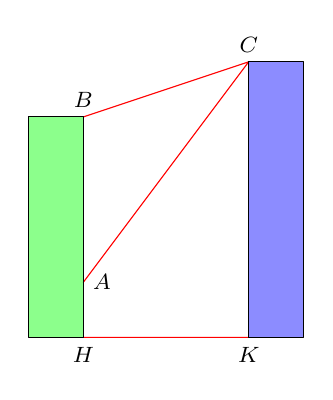
\begin{tikzpicture}[>=stealth,line join=round,line cap=round,font=\footnotesize,scale=.7]	
		\path
		(0,0) coordinate (H)node[below]{$H$}
		(-1,0) coordinate (H1)
		(0,1) coordinate (A)node[right]{$A$}
		(0,4) coordinate (B)node[above]{$B$}
		(-1,4) coordinate (B1)
		(3,0) coordinate (K)node[below]{$K$}
		(4,0) coordinate (K1)
		(3,5) coordinate (C)node[above]{$C$}
		(4,5) coordinate (C1)
		;
		\fill[green!45]
		(H)--(B)--(B1)--(H1)--cycle
		;
		\fill[blue!45]
		(C)--(K)--(K1)--(C1)--cycle
		;
		\draw[red]
		(B)--(C)
		(A)--(C)
		(H)--(K)
		;
		\draw[black]
		(H)--(B)--(B1)--(H1)--cycle
		(C)--(K)--(K1)--(C1)--cycle
		;
		\end{tikzpicture}
	\end{center}
	\loigiai{
		\immini{Ta có $CD=CK-BH=8$, $CI=CK-AH=26$, $BD=AI=HK=20$.\\
			$\tan\widehat{BCD}=\dfrac{BD}{CD}=\dfrac{20}{8}=\dfrac{5}{2}$, $\tan\widehat{ACI}=\dfrac{AI}{CI}=\dfrac{20}{26}=\dfrac{10}{13}$.\\
			$\tan\widehat{BCA}=\tan\left(\widehat{BCD}-\widehat{ACI}\right)=\dfrac{\tan\widehat{BCD}-\tan\widehat{ACI}}{1+\tan\widehat{BCD}.\tan\widehat{ACI}}=\dfrac{\frac{5}{2}-\frac{10}{13}}{1+\frac{5}{2}\cdot\frac{10}{13}}$\\
			$\tan\widehat{BCA}=\dfrac{45}{76}\Rightarrow \widehat{BCA}\approx 30,6^\circ $.
			
		}
		{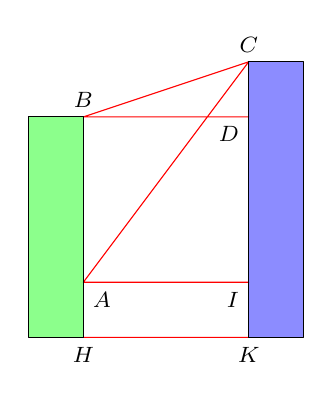
\begin{tikzpicture}[>=stealth,line join=round,line cap=round,font=\footnotesize,scale=.7]	
			\path
			(0,0) coordinate (H)node[below]{$H$}
			(-1,0) coordinate (H1)
			(0,1) coordinate (A)node[below right]{$A$}
			(0,4) coordinate (B)node[above]{$B$}
			(-1,4) coordinate (B1)
			(3,0) coordinate (K)node[below]{$K$}
			(4,0) coordinate (K1)
			(3,5) coordinate (C)node[above]{$C$}
			(4,5) coordinate (C1)
			(3,4) coordinate (D)node[below left]{$D$}
			(3,1) coordinate (I)node[below left]{$I$}
			;
			\fill[green!45]
			(H)--(B)--(B1)--(H1)--cycle
			;
			\fill[blue!45]
			(C)--(K)--(K1)--(C1)--cycle
			;
			\draw[red]
			(B)--(C)
			(A)--(C)
			(H)--(K)
			(B)--(D)
			(A)--(I)
			;
			\draw[black]
			(H)--(B)--(B1)--(H1)--cycle
			(C)--(K)--(K1)--(C1)--cycle
			;
			\end{tikzpicture}
		}
	}	
\end{ex}

\begin{ex}%[1D1V3-4]%[Dự án đề cương 3 Khối NH 24-25- Dot 3- Nguyễn Trần Anh Tuấn]
	Khi nhấn một phím trên điện thoại cảm ứng, bàn phím sẽ tạo ra hai âm thuần, kết hợp với nhau để tạo ra âm thanh nhận dạng duy nhất phím. Hình vẽ bên dưới cho thấy tần số thấp $f_1$ và tần số cao $f_2$ liên quan đến mỗi phím. Nhấn một phím sẽ tạo ra sóng âm $y=\sin \left(2 \pi f_1 t\right)+\sin \left(2 \pi f_2 t\right)$, ở đó $t$ là biến thời gian (tính bằng giây).
	\begin{center}
		\begin{tikzpicture}[scale=1.3,>=stealth, font=\footnotesize, line join=round, line cap=round]
			\def\xmin{-6} \def\xmax{6}
			\def\ymin{-8} \def\ymax{8} 
			%	\draw[color=gray!50,dashed] (\xmin,\ymin) grid (\xmax,\ymax); 
			%	\clip (\xmin+0.1,\ymin+0.1) rectangle (\xmax-0.5,\ymax-0.1);
			\draw (1,1) node {\fbox{$\boldsymbol1$}} (2,1) node {\fbox{$\boldsymbol2$}} (3,1) node {\fbox{$\boldsymbol3$}} (1,0) node {\fbox{$\boldsymbol4$}} (2,0) node {\fbox{$\boldsymbol5$}} (3,0) node {\fbox{$\boldsymbol6$}} (1,-1) node {\fbox{$\boldsymbol7$}} (2,-1) node {\fbox{$\boldsymbol8$}} (3,-1) node {\fbox{$\boldsymbol9$}} (1,-2) node {\fbox{\bf *}} (2,-2) node {\fbox{$\boldsymbol 0$}} (3,-2) node {\fbox{\bf\#}};
			\draw[->] (1,2) node [above]{$1209 $}->(1,1.4);
			\draw[->](2,2) node [above]{$1336 $}--(2,1.4); 
			\draw[->](3,2) node [above]{$1477~\mathrm{Hz}$}--(3,1.4);
			\draw[->] (0,1) node [left]{$697~\mathrm{Hz}$}->(.6,1);
			\draw[->] (0,0) node [left]{$770 ~\mathrm{Hz}$}->(.6,0);
			\draw[->] (0,-1) node [left]{$852~ \mathrm{Hz}$}->(.6,-1);
			\draw[->] (0,-2) node [left]{$941~ \mathrm{Hz}$}->(.6,-2);
			\draw (2,2.4) node [above]{\bf Tần số cao};
			\draw (-1.2,-.5) node [rotate=90,black]{\bf Tần số thấp};
		\end{tikzpicture}
	\end{center}
	\begin{enumerate}
		\item Tìm hàm số mô hình hoá âm thanh được tạo ra khi nhấn phím $4$.
		\item  Biến đổi công thức vừa tìm được ở câu trên về dạng tích của một hàm số sin và một hàm số côsin.
	\end{enumerate}
	\loigiai{
		\begin{enumerate}
			\item  Nhấn  phím $4$ sẽ tạo ra sóng âm $y=\sin \left(2 \pi f_1 t\right)+\sin \left(2 \pi f_2 t\right)$ với $f_{1}=770 \mathrm{\mathrm{Hz}}$ và $f_{2}=1\,209 \mathrm{Hz}$.\\
			Khi đó $y=\sin \left(2 \pi 770 t\right)+\sin \left(2 \pi 1209 t\right)$.\\
			Hay $y=\sin \left(1\,540 \pi  t\right)+\sin \left(2\,418 \pi  t\right)$.	
			\item  Ta có 
			\[
			\begin{aligned}
				y&=\sin \left(1\,540 \pi t\right)+\sin \left(2\,418 \pi t\right)\\
				&= 2\sin \dfrac{1\,540 \pi t+2\,418 \pi t}{2}\cos \dfrac{1\,540 \pi t-2\,418 \pi t}{2}\\
				&=2\sin(1\,979 \pi t)\cos (439 \pi t). 
			\end{aligned}\]
		\end{enumerate}
	}
\end{ex}

\begin{ex}%[1D1V3-4]%[Dự án đề cương 3 Khối NH 24-25- Dot 3- Nguyễn Trần Anh Tuấn]
	Hiệu điện thế và cường độ dòng điện trong một thiết bị điện lần lượt được cho bởi các biểu thức sau
	$$
	\begin{aligned}
	& u=40 \sin (120 \pi t)+10 \sin (360 \pi t)(\mathrm{V}) \\
	& i=4 \sin (120 \pi t)+\sin (360 \pi t) \quad \text { (A). }
	\end{aligned}
	$$
	\begin{flushright}
		(Nguồn: Ron Larson, Intermediate Algebra, Cengage)
	\end{flushright}
	Biết rằng công suất tiêu thụ tức thời của thiết bị đó được tính theo công thức: $P=u \cdot i$ (W). Hãy viết biểu thức biểu thị công suất tiêu thụ tức thời ở dạng không có lũy thừa và tích của các biểu thức lượng giác.
	\loigiai{
		Ta có
		$$
		\begin{aligned}
		P & =u \cdot i=[40 \sin (120 \pi t)+10 \sin (360 \pi t)] \cdot[4 \sin (120 \pi t)+\sin (360 \pi t)] \\
		& =160 \sin ^{2}(120 \pi t)+10 \sin ^{2}(360 \pi t)+80 \sin (120 \pi t) \sin (360 \pi t) \\
		& =80[1-\cos (240 \pi t)]+5[1-\cos (720 \pi t)]+40[\cos (360 \pi t-120 \pi t)-\cos (360 \pi t+120 \pi t)] \\
		& =85-80 \cos (240 \pi t)-5 \cos (720 \pi t)+40 \cos (240 \pi t)-40 \cos (480 \pi t) \\
		& =85-40 \cos (240 \pi t)-5 \cos (720 \pi t)-40 \cos (480 \pi t)(\mathrm{W}).
		\end{aligned}
		$$	
	}
\end{ex}